\documentclass[eng,openany]{mgr}
\usepackage{listings}
\usepackage[english]{babel}
\usepackage{graphicx}
\usepackage{hyperref}
\usepackage{tabularx,colortbl} 
\usepackage{rotating}
\usepackage[utf8]{inputenc} 
\setlength\parindent{24pt}
\usepackage[parfill]{parskip}
\usepackage[table,kernelfbox,hyperref]{xcolor}
\usepackage{fancyhdr}
\usepackage{gauss}
%\usepackage[colorinlistoftodos]{todonotes}

\hypersetup{colorlinks=true}
\hypersetup{xurlbordercolor=red!70!black}
\hypersetup{xlinkbordercolor=blue!70!black}
\hypersetup{linkcolor=blue!60!black}
\hypersetup{urlcolor=red!50!black}
\hypersetup{citecolor=green!30!black}
\rfoot{Page \thepage}
\renewcommand\lstlistlistingname{List of Listings}
\newcommand{\linia}{\rule{\linewidth}{0.4mm}}

\definecolor{listlightgray}{gray}{0.93}

\newcommand{\lstsetmylst} {
\lstset{frame = tb,
breaklines=true,
framerule = 0.25pt,
float,
fontadjust,
backgroundcolor={\color{listlightgray}},
basicstyle = {\ttfamily\footnotesize},
identifierstyle = {\ttfamily},
stringstyle = {\ttfamily},
showstringspaces = false,
showtabs = false,
numbers = left,
numbersep = 6pt,
tabsize = 4,
language=C,
floatplacement=!h
}
}

\newcommand{\lstsetatc} {
\lstset{frame = tb,
breaklines=true,
framerule = 0.25pt,
float,
fontadjust,
backgroundcolor={\color{listlightgray}},
basicstyle = {\ttfamily\footnotesize},
keywordstyle = {\ttfamily\color{listkeyword}\textbf},
identifierstyle = {\ttfamily},
commentstyle = {\ttfamily\color{listcomment}\textit},
stringstyle = {\ttfamily},
showstringspaces = false,
showtabs = false,
numbers = left,
numbersep = 6pt,
numberstyle={\ttfamily\color{listnumbers}},
tabsize = 4,
language=C,
floatplacement=!h
}
}

\newcommand{\lstsetatbashnum} {
\lstset{frame = tb,
breaklines=true,
framerule = 0.25pt,
aboveskip=2ex,
float,
fontadjust,
backgroundcolor={\color{listlightgray}},
basicstyle = {\ttfamily\footnotesize},
keywordstyle = {\ttfamily\color{listkeyword}\textbf},
identifierstyle = {\ttfamily},
commentstyle = {\ttfamily\color{listcomment}\textit},
stringstyle = {\ttfamily},
showstringspaces = false,
showtabs = false,
numbers = left,
numbersep = 6pt,
numberstyle={\ttfamily\color{listnumbers}},
tabsize = 4,
language=bash,
floatplacement=!h
}
}
\lstsetmylst
\author{Jaroslaw M. Szumega}
\title{}
\engtitle{}
\supervisor{Rafal Zdunek, D.Sc, K-4/W4}
\field{Electronics}
\specialisation{Advanced Applied Electronics}
\date{20.03.2017}
\begin{document}
\selectlanguage{english}
\maketitle

\newpage

\chapter{Solution to the given problems}
(Problems 1, 3, 4 and 7 are solved analytically, without using any of selected algorithms. Result are checked with built-in Octave/Matlab function.)

\textbf{Problem 1} - Compute the eigenpairs of the matrices. Verify that trace equals to eigenvalues sum and the determinant to their product. Which matrix is singular?

To find eigenvalues, the following calculations will be used:\\
\begin{math}
Ax - \lambda x = 0 \\
(A - \lambda I) x = 0 \\
det(A - \lambda I) = 0
\end{math}
Then the characteristic polynomial can be determined. It's roots are the eigenvalues.

\textbf{Matrix A1}

\[
A_1 =
\begin{bmatrix}
1 & 0 & 0  \\
2 & 1 & 0 \\
0 & 0 & 3 
\end{bmatrix}
\]

\[
det
\begin{bmatrix}
1 -\lambda & 0 & 0  \\
2 & 1-\lambda & 0 \\
0 & 0 & 3-\lambda 
\end{bmatrix}
=(1-\lambda)(1-\lambda)(3-\lambda)
\]

\begin{math}
For \lambda = 1:\\
\begin{bmatrix}
0 & 0 & 0  \\
2 & 0 & 0 \\
0 & 0 & 2 
\end{bmatrix}
\begin{bmatrix}
x_1 \\
x_2 \\
x_3
\end{bmatrix}
= 0\; =>
\begin{matrix}
2x_1 = 0\\
2x_3 = 0\\
(no\;x_2\;formula)
\end{matrix}
=>
x = 
\begin{bmatrix}
0\\
t \\
0
\end{bmatrix}
\end{math}

\begin{math}
For \lambda = 3:\\
\begin{bmatrix}
-2 & 0 & 0  \\
2 & -2 & 0 \\
0 & 0 & 0 
\end{bmatrix}
\begin{bmatrix}
x_1 \\
x_2 \\
x_3
\end{bmatrix}
= 0\; =>
\begin{matrix}
-2x_1 = 0\\
2x_1 -2x_2 = 0\\
(no\;x_3\;formula)
\end{matrix}
=>
x = 
\begin{bmatrix}
0\\
0 \\
t
\end{bmatrix}
\end{math}
\\ \\ 
$tr(A) = 1 + 1 + 3 = 5$\\
$\sum \lambda = 1 + 1 + 3 = 5
\\ \\
det(A) = 1 \cdot 1 \cdot 3$ = 3\\
$\prod \lambda = 1 \cdot 1 \cdot 3$ = 3
\\
Matrix determinant is non--zero, so the matrix is not singular.
\newpage
\textbf{Matrix A2}
\[
A_2 =
\begin{bmatrix}
	0 & -2 & 1  \\
	1 & 3 & -1 \\
	0 & 0 & 1 
\end{bmatrix}
\]

\[
det
\begin{bmatrix}
0-\lambda & -2 & 1  \\
1 & 3-\lambda & -1 \\
0 & 0 & 1-\lambda 
\end{bmatrix}
= (Sarrus\;theorem =>)(1-\lambda)(1-\lambda)(3-\lambda) = \\ 
\]
\[
= (-\lambda)(3-\lambda)(1-\lambda) - (-2)(1-\lambda) = (1-\lambda)(\lambda ^2 - 3\lambda + 2)
\]

\begin{math}
For \lambda = 1:\\
\begin{bmatrix}
-1 & -2 & 1  \\
1 & 2 & -1 \\
0 & 0 & 0 
\end{bmatrix}
\begin{bmatrix}
x_1 \\
x_2 \\
x_3
\end{bmatrix}
= 0\; =>
\begin{matrix}
-x_1 -2x_2+x_3 = 0\\
x_1+2x_2-x_3 = 0\\

\end{matrix}
=>
x = 
\begin{bmatrix}
-2v_2+v_3\\
v_2 \\
v_3
\end{bmatrix}
\end{math}

\begin{math}
For \lambda = 2:\\
\begin{bmatrix}
-2 & -2 & 1  \\
1 & 1 & -1 \\
0 & 0 & -1 
\end{bmatrix}
\begin{bmatrix}
x_1 \\
x_2 \\
x_3
\end{bmatrix}
= 0\; =>
\begin{matrix}
-2x_1 -2x_2+x_3 = 0\\
x_1+x_2-x_3 = 0\\
(-x_3=0)
\end{matrix}
=>
x = 
\begin{bmatrix}
v\\
-v \\
0
\end{bmatrix}
\end{math}
\\ \\ 
$tr(A) = 3 +1 = 4$\\
$\sum \lambda = 1+1+2 = 4
\\ \\
det(A) = 2\\
\prod \lambda = 1 \cdot 1 \cdot 2$ = 2
\\
Matrix determinant is non--zero, so the matrix is not singular.
\\
\\
\textbf{Matrix A3}
\[
A_3 =
\begin{bmatrix}
	4 & 1 & 0  \\
	1 & 4 & 1 \\
	0 & 1 & 4 
\end{bmatrix}
\]

\[
de
A_3 =
\begin{bmatrix}
4-\lambda & 1 & 0  \\
1 & 4-\lambda & 1 \\
0 & 1 & 4-\lambda 
\end{bmatrix}t
= (Sarrus\;theorem =>)(4-\lambda)(4-\lambda)(4-\lambda)- (4-\lambda) - (4-\lambda) = 
\]
\[
= (4-\lambda)(\lambda^2 - 8 \lambda + 14) = (4-\lambda)(\lambda - (4+\sqrt{2}))(\lambda - (4-\sqrt{2}))
\]

\begin{math}
For \lambda = 4:\\
\begin{bmatrix}
0 & 1 & 0  \\
1 & 0 & 1 \\
0 & 1 & 0 
\end{bmatrix}
\begin{bmatrix}
x_1 \\
x_2 \\
x_3
\end{bmatrix}
= 0\; =>
\begin{matrix}
-x_1 -2x_2+x_3 = 0\\
x_1+2x_2-x_3 = 0\\

\end{matrix}
=>
x = 
\begin{bmatrix}
-2v_2+v_3\\
v_2 \\
v_3
\end{bmatrix}
\end{math}

\begin{math}
For \lambda = 4+\sqrt{2}:\\
\begin{bmatrix}
-\sqrt{2} & 1 & 0  \\
1 & -\sqrt{2} & -1 \\
0 & 1 & -\sqrt{2} 
\end{bmatrix}
\begin{bmatrix}
x_1 \\
x_2 \\
x_3
\end{bmatrix}
= 0\; =>
\begin{matrix}
-\sqrt2x_1 +x_2 = 0\\
x_1-\sqrt2x_2+x_3 = 0\\
x_2-\sqrt2x_3=0
\end{matrix}
=>
x = 
\begin{bmatrix}
v\\
\sqrt2v \\
v
\end{bmatrix}
\end{math}

\begin{math}
For \lambda = 4-\sqrt{2}:\\
\begin{bmatrix}
\sqrt{2} & 1 & 0  \\
1 & \sqrt{2} & -1 \\
0 & 1 & \sqrt{2} 
\end{bmatrix}
\begin{bmatrix}
x_1 \\
x_2 \\
x_3
\end{bmatrix}
= 0\; =>
\begin{matrix}
\sqrt2x_1 +x_2 = 0\\
x_1+\sqrt2x_2+x_3 = 0\\
x_2+\sqrt2x_3=0
\end{matrix}
=>
x = 
\begin{bmatrix}
v\\
-\sqrt2v \\
v
\end{bmatrix}
\end{math}
\\ \\ 
$tr(A) = 4+4+4 = 12$\\
$\sum \lambda = 4 + 4 + \sqrt2 + 4 - \sqrt2 = 12
\\ \\
det(A) = 56\\
\prod \lambda = 4 \cdot (4+\sqrt2) \cdot (4+\sqrt2) = 4 \cdot (4^2-(\sqrt2)^2)= 4 \cdot 14 = 56$
\\
Matrix determinant is non--zero, so the matrix is not singular.

\textbf{Matrix A4}
\[
A_4 =
\begin{bmatrix}
1 & 2 & 3 & 4\\
5 & 6 & 7 & 8\\
9 & 10 & 11 & 12\\
13 & 14 & 15 & 16
\end{bmatrix}
\begin{matrix}
R2-2R1 \\
R3-R1\\
=\\
R4-4R1\\
&
\end{matrix}
\begin{bmatrix}
1 & 2 & 3 & 4\\
3 & 2 & 1 & 0\\
6 & 4 & 2 & 0\\
9 & 6 & 3 & 0
\end{bmatrix}
\begin{matrix}
 \\
R3-2R2\\
=\\
R4-3R2\\
&
\end{matrix}
\begin{bmatrix}
1 & 2 & 3 & 4\\
3 & 2 & 1 & 0\\
0 & 0 & 0 & 0\\
0 & 0 & 0 & 0
\end{bmatrix}
\]
det(A) = 0, so matrix is singular.
\\
\\
Now calculating the eigenvalues:\[
\begin{bmatrix}
1-\lambda & 2 & 3 & 4\\
5 & 6-\lambda & 7 & 8\\
9 & 10 & 11-\lambda & 12\\
13 & 14 & 15 & 16-\lambda
\end{bmatrix}
=>
\begin{matrix}
& \lambda_1 = 0\\
& \lambda_2 = 0\\
& \lambda_3 = 17+3\sqrt{41}\\
&\lambda_4 = 17-3\sqrt{41}\\
\end{matrix}
\]
\\ \\ 
$tr(A) = 1+6+11+16 = 34 = 12\\
\sum \lambda = 0 + 0 + 17 +3\sqrt{41}+17-3\sqrt{31} = 34
\\ \\
det(A) = 0\\
\prod \lambda = 0$
\\
Matrix determinant is zero, so the matrix is singular.
\newpage
\begin{figure}[h]
\centering
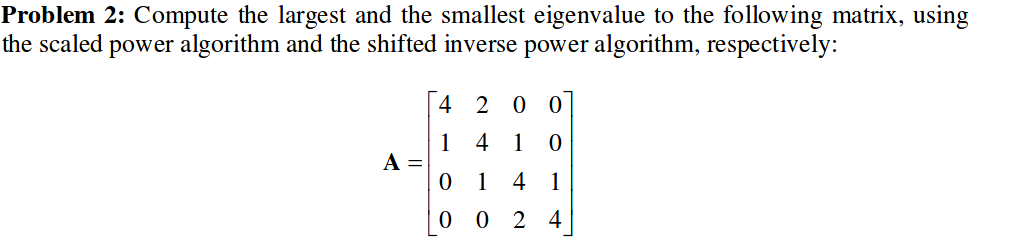
\includegraphics[width=0.8\linewidth]{screenshot001}
\label{fig:screenshot001}
\end{figure}
To compute the required values, the Scaled Power algorithm (Alg.1) and the shift inverse Power algorithm (Alg.2) were coded.

The task solution was designed in the following Octave code:
\begin{lstlisting}
A = [4 2 0 0; 1 4 1 0; 0 1 4 1; 0 0 2 4]
iterations = 10;
#computing the biggest and smallest eigenpairs

disp(['Eigenproblems using Power methods:'])

[eigenvalueMAX, eigenvectorMAX] = scaledpower(A, iterations)
[eigenvalueMIN, eigenvectorMIN] = inversepower(A, iterations)
\end{lstlisting}

That gave the results:
\begin{figure}[h]
\centering
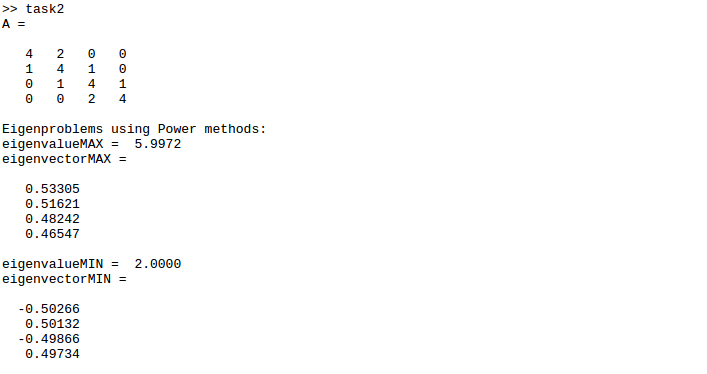
\includegraphics[width=0.8\linewidth]{screenshot002}
\label{fig:screenshot002}
\end{figure}

As it can be compared, after 10 iterations they are quite correct approximation of the exact values:
\begin{figure}[h]
\centering
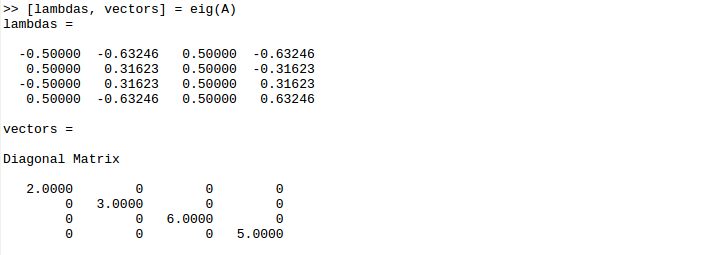
\includegraphics[width=0.8\linewidth]{screenshot003}
\label{fig:screenshot003}
\end{figure}
\newpage
\begin{figure}[h]
\centering
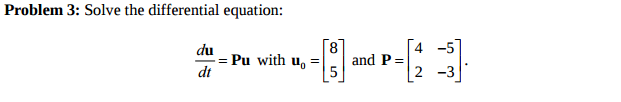
\includegraphics[width=0.8\linewidth]{screenshot004}
\label{fig:screenshot004}
\end{figure}
Solution of the differential equation has the following form:
\begin{center}
$u = \alpha \cdot exp\{\lambda t\}$\\
\end{center}
So in this particular case we are looking for:\\
$u_1 = \alpha_1 \cdot exp\{\lambda_1 t\}$\\
$u_2 = \alpha_2 \cdot exp\{\lambda_2 t\}$
\[
\begin{bmatrix}
4& -5\\
2& -3\\
\end{bmatrix}
\begin{bmatrix}
\alpha_1\\
\alpha_2\\
\end{bmatrix}
= \lambda
\begin{bmatrix}
\alpha_1\\
\alpha_2\\
\end{bmatrix}
\]

Now, we are calculating the eigenvalues:
\[
det
\begin{bmatrix}
4-\lambda&-5 \\
2& -5-\lambda\\
\end{bmatrix}
= (4-\lambda)(-3-\lambda)+10 = -12 -4\lambda +3\lambda + \lambda^2 + 10 = \lambda^2 = \lambda -2 = (\lambda-2)(\lambda+1)
\]

$For \lambda=2:$
\[
\begin{bmatrix}
2 & -5\\
2 & -5
\end{bmatrix}
\begin{bmatrix}
x_1\\
x_2
\end{bmatrix}
= 0 =>
\begin{matrix}
2x_1 - 5x_2 = 0&\\
so\; 2x_1 = 5x_2&
\end{matrix}
=> x =
\begin{bmatrix}
 5t\\
 2t
\end{bmatrix}
\]

$For \lambda=-1$:
\[
\begin{bmatrix}
5 & -5\\
2 & -2
\end{bmatrix}
\begin{bmatrix}
x_1\\
x_2
\end{bmatrix}
= 0 =>
\begin{matrix}
5x_1 = 5x_2&\\
so \; x_1 = x_2&
\end{matrix}
=> x =
\begin{bmatrix}
t\\
t
\end{bmatrix}
\]

And now the solution is in the following form:
\[
u = c_1 exp\{2t\}
\begin{bmatrix}
5\\
2
\end{bmatrix}
+ c_2 exp\{-t\}
\begin{bmatrix}
1\\
1
\end{bmatrix}
\]
Using initial condition the c values will be calculated (assuming eigenvector for t=1).
\[
\begin{bmatrix}
5 & 1\\
2 & 1
\end{bmatrix}
\begin{bmatrix}
c_1\\
c_2
\end{bmatrix}
=
\begin{bmatrix}
8\\5
\end{bmatrix}
=> 
\begin{matrix}
5c_1+c_2 = 8\\
2c_1+c_2 = 5
\end{matrix}
=>
\begin{matrix}
c_1 = 1\\
c_2 = 3
\end{matrix}
\]

Assembling all calculations, the solution to the differential equation is:
\[
u = 1\cdot exp\{2t\}
\begin{bmatrix}
5\\2
\end{bmatrix}
+
3\cdot exp\{-t\}
\begin{bmatrix}
1\\1
\end{bmatrix}
\]
\newpage
\begin{figure}[h]
\centering

\includegraphics[width=0.8\linewidth]{screenshot005}
\label{fig:screenshot005}
\end{figure}
Matrix can be diagonalized, if it has an inverse. So at first the determinant must be non-zero.

$det(A) = 4\cdot2 - 3\cdot1 = 5$

The eigenvalues need to be calculated
\[
det
\begin{bmatrix}
4-\lambda&3\\
1 & 2-\lambda
\end{bmatrix}
= (4-\lambda)(2-\lambda)-3 = 8 - 4\lambda -2\lambda + \lambda^2 -3 = (\lambda-1)(\lambda-5)
\] 

$For \lambda=1$:
\[
\begin{bmatrix}
3 & 3\\
1 & 1
\end{bmatrix}
\begin{bmatrix}
x_1\\
x_2
\end{bmatrix}
= 0 =>
\begin{matrix}
3x_1 + 3x_2 = 0&\\
x_1 = -x_2&
\end{matrix}
=> x_1 =
\begin{bmatrix}
1\\
-1
\end{bmatrix}
\]
$For \lambda=5$:
\[
\begin{bmatrix}
-1 & 3\\
1 & -3
\end{bmatrix}
\begin{bmatrix}
x_1\\
x_2
\end{bmatrix}
= 0 =>
\begin{matrix}
-x_1 + 3x_2 = 0&\\
x_1 - 3x_2 = 0&
\end{matrix}
=> x_1 = 3x_2
=>
x_2=
\begin{bmatrix}
3\\
1
\end{bmatrix}
\]

Now to calculate $A^{100}$ we will use the following formula:\\
\[
A^{100} = X \Lambda^k X^{-1}
\]
And to calculate $\Lambda$ itself:
\[
\\
\Lambda = X^{-1}AX
\]
The matrices:\[
X = 
\begin{bmatrix}
1 &3\\
-1 & 1
\end{bmatrix}
\; \; \;\; \; \;
X^{-1} = 
\begin{bmatrix}
0.25 &-0.75\\
0.25 & 0.25
\end{bmatrix}
\; \; \;\; \; \;
\Lambda =
\begin{bmatrix}
1 &0\\
0 & 5
\end{bmatrix}
\]

And the final calculation:
\[
A^{100} = X \Lambda^{100} X^{-1} = 
\begin{bmatrix}
1 &3\\
-1 & 1
\end{bmatrix}
\begin{bmatrix}
1 &0\\
0 & 5
\end{bmatrix}
^{100}
\begin{bmatrix}
0.25 &-0.75\\
0.25 & 0.25
\end{bmatrix}
=
\begin{bmatrix}
   5.9165e+69&   5.9165e+69\\
   1.9722e+69&   1.9722e+69
\end{bmatrix}
\]
\newpage
\begin{figure}[h]
\centering

\includegraphics[width=0.8\linewidth]{screenshot006}
\label{fig:screenshot006}
\end{figure}
Matrix is diagonalizable if:
\begin{itemize}
	\item can be inverted,
	\item has n linearly independent eigenvectors,
	\item surely is diagonalizable if has n distinct eigenvalues.
\end{itemize}
\[
det
\begin{bmatrix}
2 &1 &1\\
2 &1 &-2\\
-1 &0 &-2
\end{bmatrix}
= 3
\]
Determinant is not equal to zero, so matrix has an inverse.
\\

Using coded "basic QR iteration" (Algorithm 3) we will search eigenvalues and eigenvectors.

\begin{lstlisting}
[l,v] = iterqr(A, 100000)
A =
2   1   1
2   1  -2
-1   0  -2

l =
Diagonal Matrix

3.0000	 0         0
0		-1.0000    0
0        0        -1.0000


v =
0.63500    0.40825    0.40825 
0.76200   -0.81650   -0.81650 
-0.12700  -0.40825   -0.40825
\end{lstlisting}

The calculations show, that the eigenvalues are not distinct -- there is a possibility that diagonal do not exists.\\
To be completely sure, the eigenspace has to be estimated.
Looking at the eigenvectors value, we can see that two of them are equal. Therefore they are linearly dependent.
\\

The conclusion is that the diagonal of the presented matrix does not exist.
\newpage
\begin{figure}[h]
\centering

\includegraphics[width=0.8\linewidth]{screenshot007}
\label{fig:screenshot007}
\end{figure}


\chapter{Listings of algorithms}
\section{Coded selected algorithms}
Algorithm 1 - Scaled Power algorithm\\
It calculates the dominant eigenvalue and eigenvector. 
\begin{lstlisting}
function [lambda, vector] = scaledpower(A, iterations)

[n,n] = size(A);

q_prev = rand(n,1);
q_prev = q_prev/norm(q_prev);

lambda = [];
q = [];

for i = 1:iterations
z = A * q_prev;
q = z/norm(z);
q_prev = q;
endfor

#calculating Rayleigh quotient
lambda = (q'*A*q)/(q'*q);
vector = q;
endfunction
\end{lstlisting}
\newpage
Algorithm 2 - Inverse Power algorithm\\
In contrary to previous one - the result is the least significant eigenpair.
\begin{lstlisting}
function [lambda, vector] = inversepower(A, iterations)

[n,n] = size(A);

q_prev = rand(n,1);
q_prev = q_prev/norm(q_prev);
alpha = 1;
I = eye(n);
q = [];
v=[];
for i = 1:iterations

v = inv(A - alpha*I)*q_prev;
q = v/norm(v);
q_prev = q;
endfor

lambda = (q'*A*q)/(q'*q);
vector = q;

endfunction

\end{lstlisting}
Algorithm 3 - Basic QR iterations\\
Algorithm calculates the eigenvalue and eigenvectors (based on all Q product).
\begin{lstlisting}
function [lambda, vector] = iterqr(A, iterations)

[n,n] = size(A);
Qproduct = eye(n,n);

for i = 1:iterations
[Q,R] = QRgivens_lecture(A);    #calculating QR
A = R*Q;                		# assigning next step A

Qproduct = Qproduct*Q;    		# eigenvectors are product of all Qs

endfor

lambda = diag(diag(A));
vector = Qproduct;

endfunction
\end{lstlisting}
\newpage
Algorithm 4 - Shift QR algorithm\\
Algorithm calculates the eigenvalue and eigenvectors (based on all Q product).
\begin{lstlisting}
function [lambda, vector] = iterqr_shift(A, iterations)

[n,n] = size(A);

Qproduct = eye(n);
I = eye(n);


for i = 1:iterations
s = A(n,n);                       #choose the element for shift
shift = s*I;                      #create shifting diagonal

[Q,R] = QRgivens_lecture(A-shift);#apply QR factorization
A = R*Q+shift;

Qproduct = Qproduct*Q;            #multiply Q product by new Q

endfor

lambda = diag(diag(A));
vector = Qproduct;
endfunction
\end{lstlisting}
\begin{thebibliography}{8}
\addcontentsline{toc}{chapter}{Bibliography}
%\addcontentsline{toc}{section}{Literatura}
\bibitem{bjorck}
Björck, Åke. Numerical methods for least squares problems. Society for Industrial and Applied Mathematics, 1996.
\bibitem{golub}
Golub, Gene H., and Charles F. Van Loan. "Matrix computations, 3rd." (1996).
\bibitem{www}
Transforming a matrix to reduced row echelon form, http://www.di-mgt.com.au/matrixtransform.html
\bibitem{zdunek}
Zdunek R., Numerical Methods - lecture slides.
\end{thebibliography}

\end{document}

